\documentclass[../main.tex]{subfiles}
\begin{document}
Lo scripting in \code{bash} è utile per automatizzare compiti ripetitivi, combinando i comandi che abbiamo già visto e che da soli non 
sempre possono fare quello che ci serve.

Uno script è un file di testo che contiene dei comandi shell. Un file di questo tipo ha estensione \code{.sh} ma \underline{può anche
essere omessa}.

\textbf{Nota:} Bash è un \underline{linguaggio interpretato}. In caso di errori quindi lo script andrà avanti.

\vspace{0.5cm}
\subsection{Primi passi}
\begin{lstlisting}[style=bash]
    #!/bin/bash

    # Questo è un commento, e inizia con il cancelletto
    echo “Ciao mondo”
\end{lstlisting}
\begin{itemize}
    \item La prima linea di codice specifica che si sta utilizzando \code{bash}
    \item I commenti si fanno utilizzando il carattere \code{\#}
    \item Uno script può essere eseguito in due modi 
    \begin{itemize}
        \item \code{bash script.sh}
        \item \code{./script.sh} (solo con permessi di esecuzione)
        \item \code{script} (solo se lo script è nella directory \code{/bin}, accessibile solo da amministratore)
    \end{itemize}
\end{itemize}

\vspace{0.5cm}
\subsection{Variabili}
Le variabili possono essere solo \textbf{interi}, \textbf{stringhe}, o \textbf{array}, \code{bash} \underline{non supporta i numeri decimali}.
\begin{lstlisting}[style=bash]
    #!/bin/bash
    i=4
    x="ciao mondo"
    echo $x
\end{lstlisting}
\textbf{Nota:} non ci sono spazi intorno a \code{=}.

\textbf{Nota:} il carattere \code{\$} espande la variabile e ne restituisce il valore, questa operazione ha la precedenza sul globbing.
Per utilizzare invece il carattere '\$' si usa \code{\textbackslash\$} o si mette la stringa tra singoli apici.

\subsubsection{Variabili predefinite}
\begin{itemize}
    \item \code{\$0}, il nome dello script
    \item \code{\$1 .. \$n}, i parametri (per parametri > 10 usare \code{\$\{nn\}})
    \item \code{\$\#}, il numero dei parametri
    \item \code{\$@}, tutti i parametri (è un array)
    \item \code{\$\$}, il PID del processo della shell corrente
    \item \code{\$!}, il PID dell'ultimo processo mandato in background
    \item \code{\$?}, il valore di ritorno dell'ultimo comando eseguito (\code{0 = true}, altrimenti ha dato errore)
\end{itemize}
\textbf{Nota:} le variabili predefinite si possono sovrascrivere assegnando un altro valore.

\textbf{Nota:} con il comando \code{exit} si esce dallo script, possiamo specificare se il programma è andato a buon fine usando ad esempio
\code{exit 0} per la buona riuscita e \code{exit 1} per un uscita che ha generato errori.


\pagebreak
\subsection{Shift}
Il comando \code{shift} sposta i valori dei parametri posizionali
\begin{figure}[h]
    \centering
    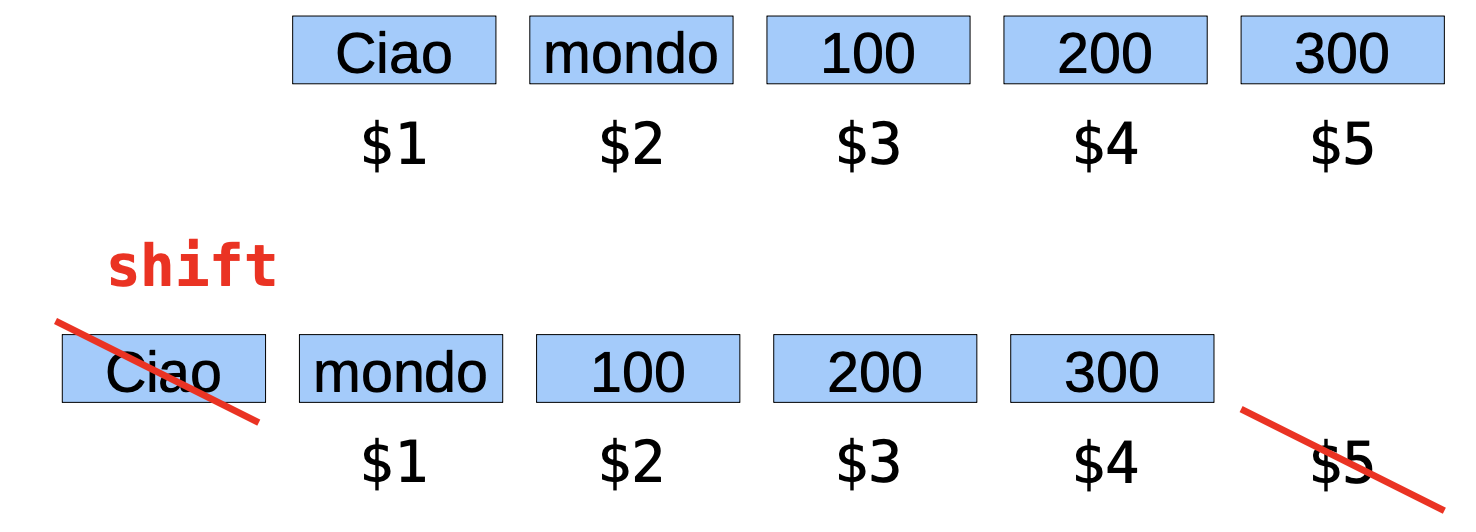
\includegraphics[width=0.7\textwidth]{../images/shift.png}
\end{figure}


\subsection{Read}
Il comando \code{read} legge l'input dell'utente e lo memorizza in una variabile
\begin{lstlisting}[style=bash]
    #!/bin/bash

    #Va a capo
    echo "Ciao come ti chiami?"
    read nome
    echo "Ciao $nome!"

    #Resta sulla riga corrente
    read -p “Come ti chiami?” nome
    echo “Ciao $nome!”

    #Resta sulla riga corrente e non mostra quello che l'untente inserisce da tastiera
    read -s -p “Password?” segreto
    echo “Conosco il tuo $segreto!”
\end{lstlisting}


\end{document}